\documentclass[11pt,openany]{book}
% #1-Asignatura
% #2-Curso
% #3-Nombre
% #4-Link
% #5-Foto

\newcommand{\portada}[5]{
    \begin{titlepage}
        \begin{center}
            \vspace*{0.5cm}
            
            % Titulo con #1 lo mas grande posible
            {\Huge \textbf{#1}}

            
            \vspace{0.5cm}
            \LARGE
            Curso #2 
            
            \vspace{1cm}
            
            \Huge{\textbf{Grupo Viterbi}}

            \vspace{1cm}
            
\includegraphics[width=0.6\textwidth]{assets/Img/UGR-Logo.png}
            
            \vspace{0.5cm}

            \huge
            PRÁCTICA 5- PROGRAMACIÓN DINÁMICA
            
            \Large
            \vspace{1cm}
            \textbf{Integrantes:}  \\ 
             % Array con los nombres de los integrantes y el correo
             \begin{center}
                \begin{tabular}{c c }
                    \textbf{Miguel Ángel De la Vega Rodríguez} & miguevrod@correo.ugr.es \\
                    \textbf{Alberto De la Vera Sánchez} & joaquinrojo724@correo.ugr.es \\
                    \textbf{Joaquín Avilés De la Fuente} & adelaveras01@correo.ugr.es \\
                    \textbf{Manuel Gomez Rubio} & e.manuelgmez@go.ugr.es \\
                    \textbf{Pablo Linari Perez} & e.pablolinari@go.ugr.es
                \end{tabular}
             \end{center}
            \vspace{0.8cm}
            
            
            \large
             \vspace{1cm}
            Facultad de Ciencias UGR\\
            Escuela Técnica Ingeniería Informática UGR\\
            Granada\\
            #2 
            
        \end{center}
    \end{titlepage}
}



\usepackage{assets/formulas}
\hbadness=10000 % Suppress Underfull \hbox warnings

%========================================|Indice|===============================================%

\begin{document}
\portada{Algorítmica}{2023-2024}{Miguel Ángel De la Vega Rodríguez}{https://github.com/Miguevrgo/}{github.png}
\tableofcontents % Índice
\newpage %Salto de pagina tras el Indice


%======================================|Documento|==============================================%
\chapter{Autores}
\begin{itemize}
    \item \textbf{Miguel Ángel De la Vega Rodríguez:} 20\%
          \begin{itemize}
              \item Plantilla y estructura del documento \LaTeX
          \end{itemize}
    \item \textbf{Joaquín Avilés De la Fuente:} 20\%
          \begin{itemize}
            \item Tarea
          \end{itemize}
    \item \textbf{Alberto De la Vera Sánchez: } 20\%
          \begin{itemize}
            \item Tarea
          \end{itemize}
    \item \textbf{Manuel Gomez Rubio} 20\%
          \begin{itemize}
            \item Tarea
          \end{itemize}
    \item \textbf{Pablo Linari Pérez:} 20\%
          \begin{itemize}
            \item Tarea
          \end{itemize}
\end{itemize}

\chapter{Objetivos}
En esta práctica, se pretende resolver problemas de forma eficiente aplicando la técnica de
Divide y Vencerás. Para ello, se han planteado varios problemas cuya solución es conocida
(excepto para el problema del viajante), y se han implementado algoritmos que los resuelven
mediante el método convencional y mediante la técnica de Divide y Vencerás. Posteriormente, se ha buscado
un umbral en el cual ambos tengan el mismo tiempo de ejecución, finalmente, se ha buscado el 
umbral óptimo para cada problema. 
\chapter{Definicion Problema}
\chapter{Algoritmo Especifico}
En este apartado, estudiaremos la eficiencia teórica, empírica e híbrida de los algoritmos especificos
de cada uno de los problemas.
\section{Problema 1: Subsecuencia de suma máxima.}
Para el primer problema, el algoritmo específico que empleamos es el algoritmo de Kadene.
\section*{Estudio teórico}
\begin{lstlisting}
      int kadane(int *a, int size){
            int max_global = a[0];
            int max_current = a[0];

            for (int i = 1; i < size; i++) {
                  max_current = max(a[i], max_current + a[i]);
                  if (max_current > max_global) {
                        max_global = max_current;
                  }
            }
            return max_global;
      }
\end{lstlisting}
Como podemos observar la eficiencia del codigo en las líneas 6-8, tienen eficiencia O(1). Por tanto,
su tiempo de ejecución es constante y notaremos por a. Luego, el bucle for se ejecutará  $(size-1)-i+1 $ 
veces, es decir, $size-i$ veces. Sabiendo que el resto de líneas del código tienen eficienciaa O(1), tenemos
el siguiente resultado
\begin{equation*}
      \sum_{i=inicial}^{size-1} a
  \end{equation*}
  Tomaremos $size =  n$ e $inicial = 1$ para simplificar el cálculo y veamos que obtenemos ahora
  \begin{equation*}\begin{split}
          \sum_{i=1}^{n-1} a = a \cdot \sum_{i=1}^{n-1} 1= a \cdot n
      \end{split}\end{equation*}
  Es claro que $a \cdot  n \in O(n)$ y por tanto la eficiencia teórica del algoritmo de kadane es $O(n)$.
  
\chapter{Algoritmo Divide y Vencerás}
En este apartado, estudiaremos la eficiencia teórica, empírica e híbrida de los algoritmos divide y vencerás
de cada uno de los problemas.
\section{Problema 1: Subsecuencia de suma máxima.}
Para el primer problema, el algoritmo específico que empleamos es 
\section*{Estudio teórico}
\begin{lstlisting}
   SumaData SumaMax (int *v, int inicio, int final){
         SumaData result, d1, d2;
         if (inicio==final){
               result.max_izq = v[inicio];
               result.max_dch = v[inicio];
               result.sum = v[inicio];
               result.max_sub = v[inicio];
               return (result);
         }

         int mid = (final+inicio)/2;
         (d1)=SumaMax(v, inicio, mid);
         (d2)=SumaMax(v, mid+1, final);
            
         result.max_izq = max(d1.max_izq, d1.sum+d2.max_izq);
         result.max_dch = max(d2.max_dch, d2.sum+d1.max_dch);
         result.sum = d1.sum + d2.sum;
         int max_cross = d1.max_dch + d2.max_izq;
         result.max_sub = max(max(max_cross, d1.max_sub), d2.max_sub);
         return (result);
   }
\end{lstlisting}
Este algoritmo devuelve un tipo de dato Suma data, un struct definido por cuatro datos de tipo int. En cuanto
a la eficiencai teórica, podemos ver una llamada recursiva a la función SumaMax con vectores de tamaño $\frac{n}{2}$. 
Teniendo en cuenta que el resto de líneas de código son asignaciones, comparaciones y operaciones arimtéticas, que son O(1), obtenemos 
la siguiente ecuación
\begin{equation*}
      T(n)=2T(\frac{n}{2})+1
\end{equation*}
Al realizar un cambio de variable $n=2^m$(luego $m=log_2(n)$), obtenemos:
\begin{gather*}
      T(2^m)=2T(2^{m-1})+1 \\
      T(2^m)-2T(2^{m-1})=1
\end{gather*}
Ahora calculamos por un lado la parte homogénea y por otro la no homogénea. En primer lugar, la homogénea:
\begin{equation*}
      T(2^m)-2T(2^{m-1})=0 \  \Longrightarrow  \ p_H(x)=x-2
\end{equation*}
En cuanto a la parte no homogénea
\begin{equation*}
      1=b_1^m q_1(m) \Longrightarrow b_1=1 \wedge q_1(m)=1 \text{ con grado } d_1=0
\end{equation*}
Tenemos entonces el siguiente polinómio característico
\begin{equation*}
    p(x)=(x-2)(x-b_1)^{d_1+1}=(x-2)(x-1)
\end{equation*}
Por tanto la solución general es
\begin{equation*}
    t_m=c_{10}2^mm^0+c_{20}1^mm^0  \overset{*}{\Longrightarrow}  t_n=c_{10}n+c_{20} \Longrightarrow T(n)=c_{10}n+c_{20}
\end{equation*}
donde en ($*$) hemos deshecho el cambio de variable \\
Por lo que obtenemos como resultado que $T(n) \in O(n)$

\section*{Estudio empírico}
\begin{figure}[h]
      \begin{minipage}{0.5\textwidth}
          \centering
          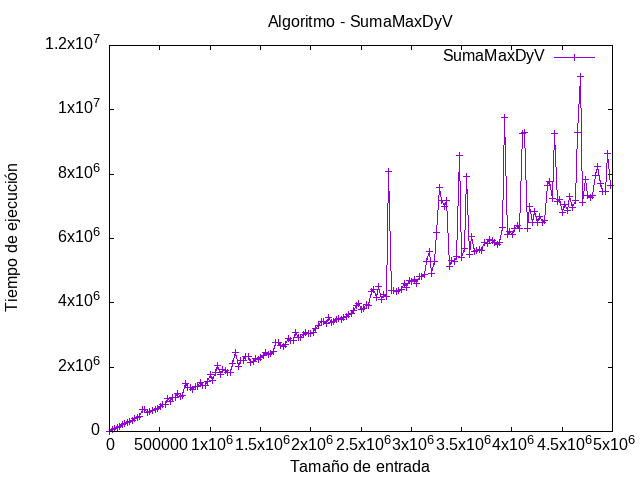
\includegraphics[width=\linewidth]{../Codigos/Graficas/SumaMaxDyV.png}
          \caption{Ejecución algoritmo SumaMaxDyV}
          \label{fig:SumaMaxDyV}
      \end{minipage}
\end{figure}


\chapter{Conclusiones}
\end{document}